% !TEX root = catron-dissertation.tex
\epstopdfsetup{outdir=./images/03_aero_optics_acoustics/}

\chapter{Aero-Optical and Acoustical Coupling}

\begin{itemize}
  \color{red}
  \item Update plots to have constant nomenclature with the rest of the document
  \item Coordinate transform between beam and duct geometry
  \item Spherical solutions and measurements
  \item Mode marching method
\end{itemize}


Acoustic waves are isentropic compression waves with the fluctuating pressure, $p'$, determining the strength of the wave.
This fluctuating pressure is related to the sound pressure level, $\spl$ by
\begin{equation}
  \spl = 20\log_{10}\left(\frac{p_{rms}}{p_0}\right)
  \label{eqn:03_spl}
\end{equation}
where $p_{rms}$ is the root mean square of the pressure fluctuation, and $p_0$ is the reference pressure (20 $\mu$Pa for air).
The pressure fluctuations can be converted to the density fluctuations via the definition of the speed of sound:
\begin{equation}
  c_0^2 = \left(\frac{\partial p}{\partial \rho}\right)_s=\frac{p'}{\rho'}
  \label{eqn:03_speed_sound}
\end{equation}
where $c_0$ is the speed of sound at mean fluid properties and the subscript $s$ denotes constant entropy.
It can be shown by combining Equations \ref{eqn:02_gladstone_dale_relation_fluctuating} and \ref{eqn:02_opd} that the fluctuating density can be related to the $\opd$,
\begin{equation}
  \opd = K_{GD}\int_{s_1}^{s_2}{\rho'}ds \textrm{.}
  \label{eqn:03_opd_fluct}
\end{equation}
This can be combined with Equation \ref{eqn:03_speed_sound},
\begin{equation}
  \opd = \frac{K_{GD}}{c_0^2}\int_{s_1}^{s_2}{p'}ds \textrm{,}
  \label{eqn:03_opd_pressure}
\end{equation}
to provide a way of computing the optical path difference of a pressure field.

When the pressure field is known in complex quantities (magnitude and phase), a complex optical path difference can calculated,
\begin{equation}
  \widehat{\opd}(x,y) = \frac{K_{GD}}{c_0^2}\int_{z_1}^{z_2} \hat{p}(x,y,z)dz \textrm{.}
  \label{eqn:03_opd_complex}
\end{equation}
Here the complex pressure field was assumed to be seperable in time and space.
The measurable $\opd$ is
\begin{equation}
  \opd(x,y) = \real\left[\sum\widehat{\opd}(x,y)\exp\{j\omega t\}\right] \textrm{.}
  \label{eqn:03_opd_real}
\end{equation}
This can greatly reduce the computational cost of simulating a beam passing through a pressue or density field that is separable in time and space by only performing the spatial integration once for each temporal frequency component.

\section{Simple Examples of Acoustic-Optical Coupling}
Two basic acoustic pressure fields will be numerically examined for their optical properties.
The first will be a planar acoustic wave that will be numerically simulated over a variety of conditions.
The second will be a spherical acoustic wave that will be both numerically simulated and validated experimentally.

\subsection{Planar Acoustic Waves}
A planar wave is the simplest solution to the wave equation and varies only in time and the direction of travel.
A planar wave can be calculated from the set of solutions for duct acoustics, Equation \ref{eqn:02_pressure_solution_duct}, given that $\Psi_m(x,y)=1$,
\begin{equation}
  \hat{p}(z,t) = p_m\exp\left\{j(\omega t \mp k_{zm}^\pm z)\right\} \textrm{.}
  \label{eqn:03_plane_wave}
\end{equation}
This section will show several plots to show the effect that acoustic waves have on the optical wavefront of a planar wave with the general geometry shown in Figure \ref{fig:03_planar_sample_domain}.
\begin{figure}
  \centering
  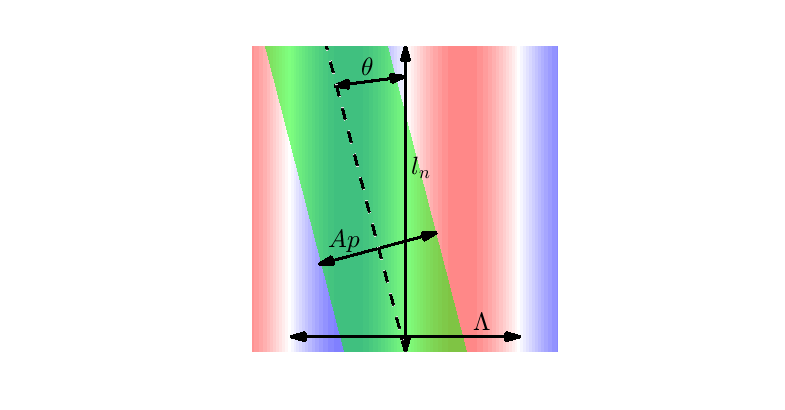
\includegraphics{../matlab/03_aero_optics_acoustics/planar_sample_domain.eps}
  \caption{General geometry for various sample calculations for showing the acoustic-optical coupling effect.}
  \label{fig:03_planar_sample_domain}
\end{figure}
For the following example, $l_n$ is the width of the acoustic disturbance (for example, the width of the wind tunnel), $\theta$ is the angle between the planar acoustic wave and the beam direction, $A_p$ is the aperture diameter of the beam, and $\Lambda$ is the wavelength of the acoustic wave.

Figure \ref{fig:03_planar_sample_calc_3} shows the time averaged $\opdrms$ per meter of beam propagation when the beam path is parallel ($\theta=0$) to the peaks and troughs of the planar acoustic wave as $\spl$ is varied.
\begin{figure}
  \centering
  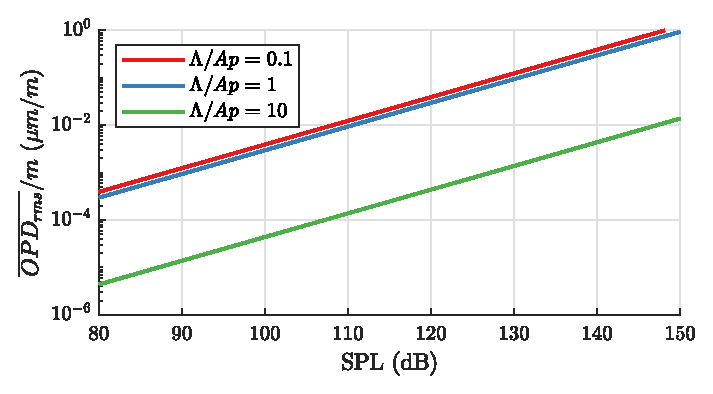
\includegraphics{../matlab/03_aero_optics_acoustics/planar_sample_calc_3.eps}
  \caption{Theoretical time-averaged $\opdrms$ per meter of beam propagation as a function of sound pressure level, $\spl$, for several $\Lambda/Ap$ ratios and $\theta=0$.}
  \label{fig:03_planar_sample_calc_3}
\end{figure}
As the sound pressure level increases the time averaged $\opdrms$ also increases and can easily reach the point of being a significant factor in the measured optical disturbance.
There is little difference between 0.1 and 1 $\Lambda/Ap$, but as the wavelength gets much larger compared to the beam diameter, then the optical effect of the noise is greatly reduced, this effect is known as aperture filtering \cite{Siegenthaler-2005-KQ2HGmfp}.

Aperture filtering is more clearly shown in Figure \ref{fig:03_planar_sample_calc_1}.
\begin{figure}
  \centering
  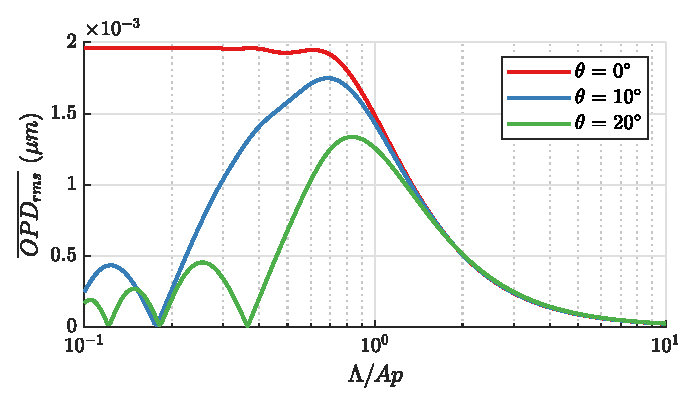
\includegraphics{../matlab/03_aero_optics_acoustics/planar_sample_calc_1.eps}
  \caption{Theoretical time-averaged $\opdrms$ for a rms sound pressure of 1 Pa ($\spl$ of 94 dB), $l_n$ of 1 m, and various angles and $\Lambda/Ap$ ratios.}
  \label{fig:03_planar_sample_calc_1}
\end{figure}
As the $\Lambda/Ap$ ratio increases from 0.1, time-averaged $\opdrms$ remains fairly constant until it starts to drop around $\Lambda/Ap$ of 0.7 and starts to asymptotically approach zero which it basically reaches by $\Lambda/Ap$ of 10.
Figure \ref{fig:03_planar_sample_calc_1} also shows the effect of changing the beam angle, $\theta$, through the acoustic field.
For nonzero $\theta$, the beam encounters alternating high and low index of refraction as it passes through the test region, so that the time-averaged $\opdrms$ begins to decrease compared to the $\theta = 0^\circ$ case below $\Lambda/Ap=1$.
There are also points of zero optical disturbance that occur at $\theta_{zero}=\tan^{-1}(n\Lambda/l_n)$ for $n\neq0$; these points occur because the peaks and valleys of the optical disturbance caused by the sound wave effectively cancel out over the length of the integration path, $l_n/\cos\theta$.

Figures \ref{fig:03_planar_sample_calc_3} and \ref{fig:03_planar_sample_calc_1} show the optical effect of plane acoustic waves in a no-flow environment.
The effect of wind-tunnel flow is to stretch (downstream-traveling waves) or compress (upstream-traveling waves) the wavelength of the acoustic noise thereby altering the filtering effect of the beam aperture.
Figure \ref{fig:03_planar_sample_calc_2} shows a typical optical disturbance from the two transverse acoustic waves (u+c and u-c) present in a wind tunnel at Mach 0.6.
\begin{figure}
  \centering
  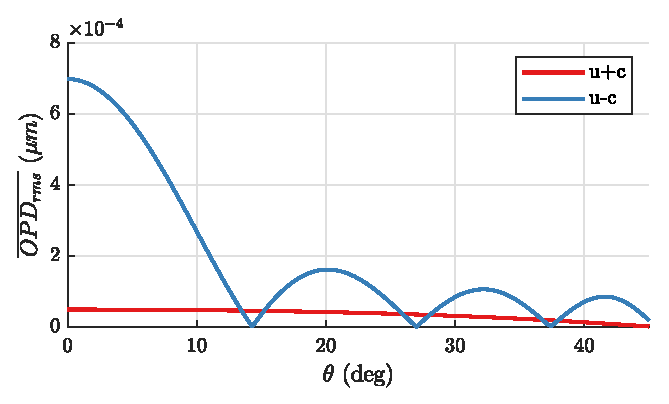
\includegraphics{../matlab/03_aero_optics_acoustics/planar_sample_calc_2.eps}
  \caption{Theoretical time-averaged $\opdrms$ for the two acoustic waves (u+c and u-c) for the blade pass frequency (534 Hz) at Mach 0.6 with a RMS sound pressure of 1 Pa ($\spl$ of 94 dB), $l_n$ of 1 m, and $Ap$ of 15 cm.}
  \label{fig:03_planar_sample_calc_2}
\end{figure}
Both waves have a RMS sound pressure of 1 Pa and the beam has an aperture of 15 cm and propagates through a 1 m acoustic field inside the tunnel.
Over a vast majority of the look back angles the upstream-traveling acoustic wave has a much greater effect on the optical disturbance compared to the downstream-traveling acoustic wave, due to the much shorter wavelength of the upstream-traveling waves which is less affected by aperture filtering.
However, the upstream-traveling wave goes through several zero points so the downstream-traveling wave dominates at some look back angles.

% In summary, Figures \ref{fig:03_planar_sample_calc_3} to \ref{fig:03_planar_sample_calc_2} give an example of how planar acoustic waves are expected to affect a beam traveling a finite distance $l_n$ at an angle $\theta$ through the acoustic field.

\subsection{Spherical Acoustic Waves}
The acoustic field from an speaker maybe assumed to be a spherical wave from a pulsating sphere if the frequency is sufficiently low and measurement region is far enough away from the source \cite{Randall-1951-9NtPPXPq}.

\begin{equation}
  \hat{p}(r,t) = \frac{A_0}{r}\exp\left\{-j(kr-\omega t)\right\}
  \label{eqn:03_spherical_pressure}
\end{equation}
% 3-16 pg61

\begin{equation}
  p_{rms} = \frac{|A_0|}{r\sqrt{2}}
  \label{eqn:03_spherical_pressure_rms}
\end{equation}

\begin{figure}
  \centering
  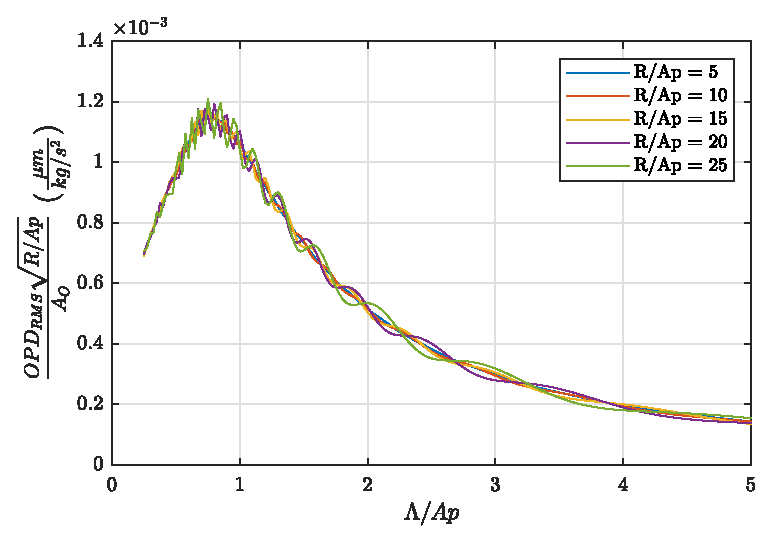
\includegraphics{../matlab/03_aero_optics_acoustics/spherical_sample.eps}
  \caption{Theoretical time-averaged $\opdrms$ for a spherical acoustic wave. There are oscillations not captured by the curve fit that are a function of aperture size.}
  \label{fig:03_spherical_sample}
\end{figure}

\begin{equation}
  \frac{\opdrms\sqrt{R/Ap}}{|A_0|} \approx \frac{p_1(\Lambda/Ap)^2+p_2(\Lambda/Ap)+p_3}{(\Lambda/Ap)^2+q_1(\Lambda/Ap)+q_2}
  \label{eqn:03_spherical_sample_fit}
\end{equation}


\begin{table}
\centering
\caption{Curve fit values for Figure \ref{fig:03_spherical_sample} and Equation \ref{eqn:03_spherical_sample_fit}}
\input{../matlab/03_aero_optics_acoustics/spherical_sample.txt}
\label{tab:03_speherical_sample_coeff}
\end{table}

\begin{table}
\centering
\caption{Comparison of microphone and wavefront computation of $|A_0|$}
\input{../matlab/03_aero_optics_acoustics/spherical_measurement.txt}
\label{tab:03_speherical_measurement}
\end{table}



\section{Estimating the Acoustic Field Inside the Test-Section}



\subsection{Mode Marching Process}
\begin{enumerate}
  \item Start with a known or assumed source acoustic field, $p^n(x,y)$

  \item Calculate the transmitted pressure ratio
  \begin{itemize}
    \item Traveling with subsonic flow
      \begin{equation}
        \frac{p^t}{p^i} = \left(\frac{1+M_n}{1+M_{n+1}}\right)\left(\frac{2M_{n+1}}{M_n+M_{n+1}}\right)\left(\frac{X_{n,n}}{X_{n,n+1}}\right)\left(\frac{X_{n,n}}{X_{n+1,n+1}}\right)^{1/(\gamma-1)}
      \end{equation}
    \item Traveling against subsonic flow
      \begin{equation}
        \frac{p^t}{p^i} = \left(\frac{1-M_n}{1-M_{n+1}}\right)\left(\frac{2M_{n+1}}{M_n+M_{n+1}}\right)\left(\frac{X_{n,n}}{X_{n,n+1}}\right)\left(\frac{X_{n,n}}{X_{n+1,n+1}}\right)^{1/(\gamma-1)}
      \end{equation}
    \item Where
      \begin{equation}
        X_{a,b} = 1+\frac{\gamma-1}{2}M_aM_b
      \end{equation}
  \end{itemize}

  \item March acoustic field to next axial step,
    \begin{equation}
      p^{n+1}(x,y) = p^{n}(x,y)\frac{p^t}{p^i}\exp\{j(\omega t\mp k_{zm}^\pm z)\}
    \end{equation}

  \item Best-fit set of local duct modes coefficients, $C_m$, to acoustic field $p^{n+1}(x,y)$

  \item Calculate new acoustic field from duct mode and repeat from step 2
    \begin{equation}
      p^n(x,y) = \sum_{m=0}^{M} C_m\cdot p_m(x,y)
    \end{equation}

  \item When the end point is reached, step inlet acoustic field (rotate fan) and repeat
\end{enumerate}
